\begin{frame}{Perfusion Analysis: Conceptual Overview}
\begin{itemize}
    \item Goal: Quantify brain tissue perfusion using Mean Transit Time (MTT)
    \item Approach: Model concentration-time curves using Gamma Variate Function (GVF)
    \item Key Assumption: Tissue response follows a gamma distribution
\end{itemize}
\end{frame}

\begin{frame}{Mathematical Framework}
\begin{align*}
    \text{GVF:} \quad C(t) &= A(t-t_0)^\alpha e^{-(t-t_0)/\beta} \\
    \text{MTT:} \quad MTT &= \alpha \beta
\end{align*}
Where:
\begin{itemize}
    \item $C(t)$: Concentration of contrast agent over time
    \item $A$: Amplitude factor
    \item $t_0$: Arrival time of contrast agent
    \item $\alpha, \beta$: Shape and scale parameters of gamma distribution
\end{itemize}
\end{frame}

\begin{frame}{Perfusion Quantification Process}
\begin{enumerate}
    \item Model tissue response: $R(t) = \frac{1}{\Gamma(\alpha)\beta^\alpha}t^{\alpha-1}e^{-t/\beta}$
    \item Assume simplified Arterial Input Function (AIF): $AIF(t) \approx \delta(t)$
    \item Tissue concentration: $C(t) = F \cdot AIF(t) \otimes R(t)$
    \item Under $\delta$-function AIF: $C(t) \approx F \cdot R(t)$
\end{enumerate}
Where $F$ is cerebral blood flow and $\otimes$ denotes convolution.
\end{frame}

\begin{frame}{Parameter Estimation}
For each voxel:
\begin{itemize}
    \item Fit GVF to observed concentration-time data
    \item Objective: Minimize error between model and observations
    \[ \min_{A,t_0,\alpha,\beta} \sum_{i=1}^{N} (C_{\text{observed}}(t_i) - C_{\text{GVF}}(t_i))^2 \]
    \item Extract MTT from fitted parameters: $MTT = \alpha \beta$
\end{itemize}
\end{frame}

\begin{frame}{Limitations and Considerations}
\begin{itemize}
    \item Simplified AIF assumption may lead to overestimation of MTT
    \item True AIF is likely also gamma-variate shaped
    \item More accurate model: $C(t) = F \cdot AIF_{\text{true}}(t) \otimes R(t)$
    \item Future work: Incorporate measured AIF for improved accuracy
\end{itemize}
\end{frame}

\begin{frame}{Results: MTT Heatmaps}
\begin{figure}
    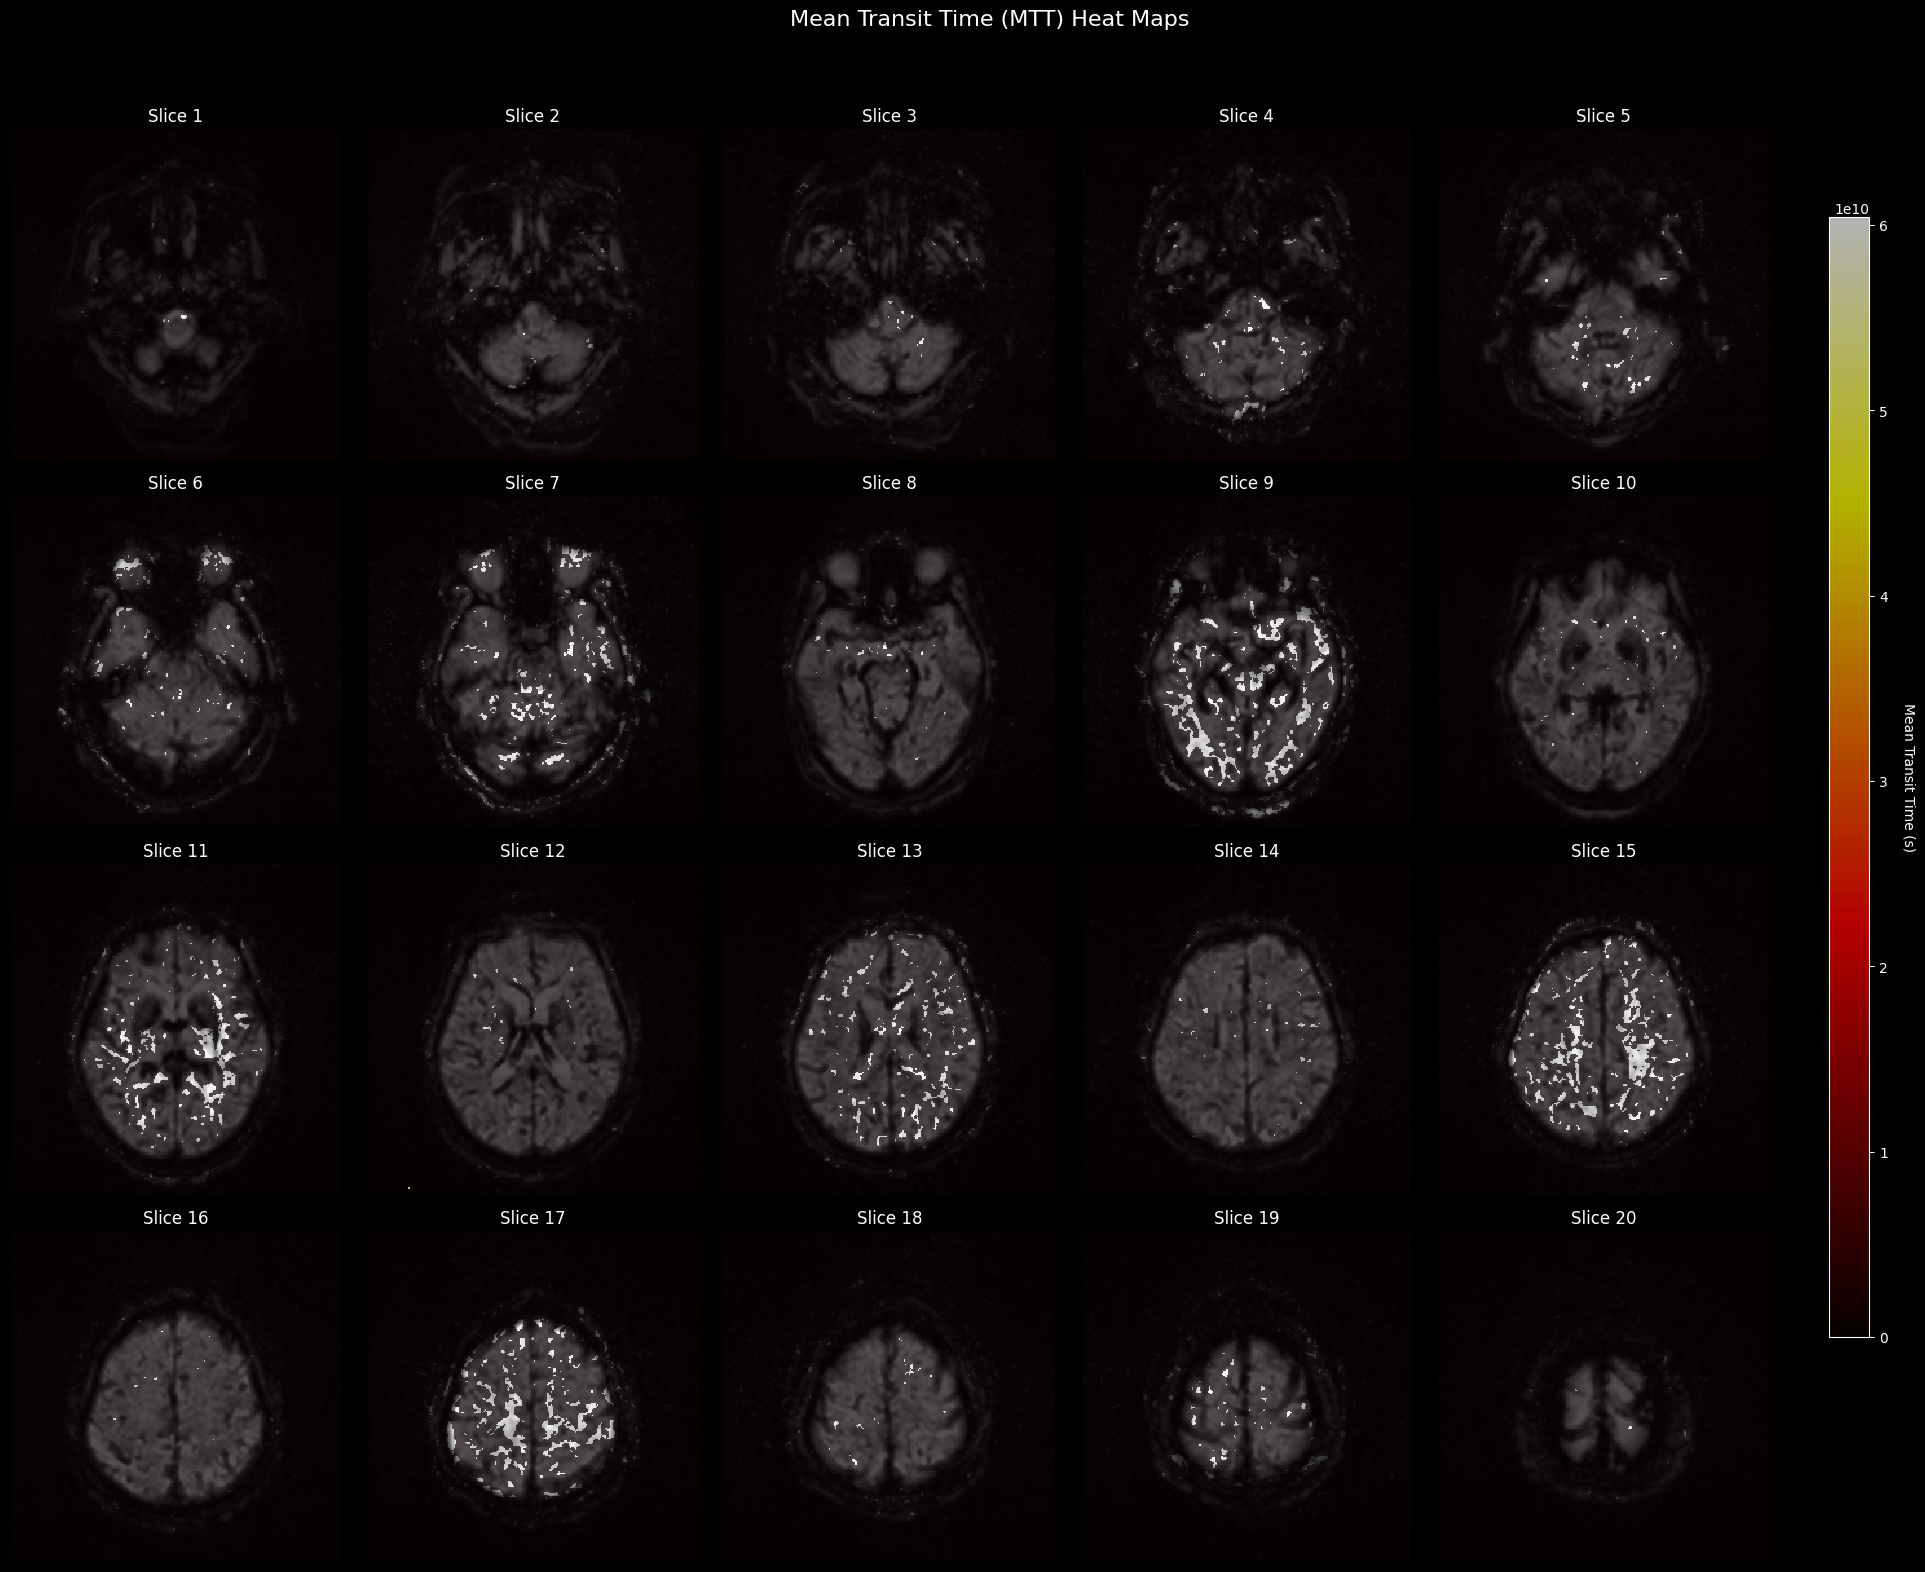
\includegraphics[width=\textwidth]{01.Oct21_GVF-MTT-HM.png}
    \caption{MTT Heatmaps overlaid on pwiMRI slices}
\end{figure}
\end{frame}